\newpage
\section{Questão 12-40}

\begin{figure}[H]
	\centering
	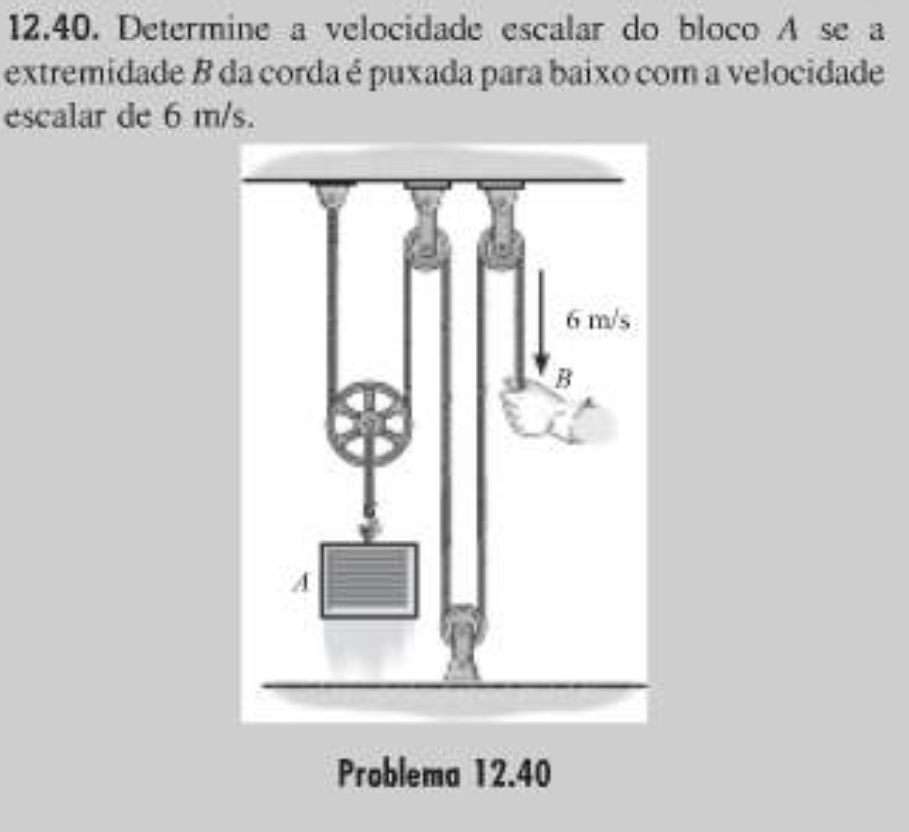
\includegraphics[width=.6\linewidth]{fundamentais/12-40.png}
	\caption{Comando da questão 12-40.}\label{fig:12-40}
\end{figure}

Nesta questão, analisamos um sistema de polias em que a velocidade no ponto \(B\) é relacionada à velocidade do bloco \(A\) devido à configuração do sistema de cordas. Determinamos a velocidade de \(A\) (\(v_A\)) quando a velocidade de \(B\) (\(v_B\)) é \(6 \, \text{m/s}\).

\subsection*{Relação entre as Velocidades}
No sistema de polias, podemos tratar os cabos como vetores de posição para identificar as velocidades relacionadas a cada elemento da seguinte forma:

\[
l_{\text{total}} = s_B + 2s_A + 2h
\]
onde:
\begin{itemize}
    \item \(s_B\): Posiçãono ponto \(B\);
    \item \(s_A\): Posição do bloco \(A\);
    \item \(h\): Altura.
\end{itemize}

\subsection*{Cálculo de \(v_A\)}
Substituímos \(v_B = 6 \, \text{m/s}\) na equação:
\[
\frac{d\left(l_{\text{total}} = s_B + 2s_A + 2h\right)}{dt} \rightarrow 0 = v_B + 2v_A
\]

Resolvendo para \(v_A\):
\[
v_A = \frac{-6}{2} = -3 \, \text{m/s}.
\]